\documentclass[slidestop,compress, 10pt]{beamer}

%\usepackage{beamerthemesplit}
\graphicspath{{Figures/}}
%\usetheme[height=1cm]{Rochester}
%\usetheme[height=1cm]{Singapore}
%\usetheme{Boadilla}
%\usetheme{boxes}
\usetheme[height=1cm]{Boadilla}
%\useoutertheme[footline=authortitle,subsection=false,height=1cm]{miniframes}
%\useoutertheme[subsection=false,height=1cm]{smoothbars}
\usepackage{epic}
%\usepackage{natbib}
%\usepackage[notocbib]{apalike}
\usepackage{color}
\beamertemplatenavigationsymbolsempty
\usepackage{graphicx}
\usepackage{color}
\usepackage[mathscr]{eucal}
\usepackage{epsfig}
\usepackage[all]{xy}
\usepackage{url}
\usepackage{setspace}
%\usepackage{xmpmulti}
\DeclareMathOperator{\E}{E}
\DeclareMathOperator{\I}{I}
\DeclareMathOperator{\Var}{Var}
\DeclareMathOperator{\Cov}{Cov}
\DeclareMathOperator{\logit}{logit}
\DeclareMathOperator{\dom}{dom}
\DeclareMathOperator{\cl}{cl}
\DeclareMathOperator{\bd}{bd}
\DeclareMathOperator{\rbd}{rbd}
\DeclareMathOperator{\intr}{int}
\DeclareMathOperator{\rint}{rint}
\DeclareMathOperator{\con}{con}
\DeclareMathOperator{\pos}{pos}
\DeclareMathOperator{\aff}{aff}
\DeclareMathOperator{\epi}{epi}
\DeclareMathOperator{\lev}{lev}
\DeclareMathOperator{\spanl}{span}

\def\RR{{\mathbb R}}
\def\ZZ{{\mathbb Z}}
\def\DD{{\mathcal D}}
\def\XX{{\mathcal X}}
\def\YY{{\mathcal Y}}
\def\TT{{\mathcal T}}
\def\NN{{\mathcal N}}
\newcommand{\deriv}[2]{\frac{d #1}{d #2}}
\newcommand{\dderiv}[2]{\frac{d^2 #1}{d #2^2}}
\newcommand{\pderiv}[2]{\frac{\partial #1}{\partial #2}}
\newcommand{\ppderiv}[2]{\frac{\partial^2 #1}{\partial #2^2}}
\newcommand{\ppmderiv}[3]{\frac{\partial^2 #1}{\partial #2 \partial #3}}
\newcommand{\fatdot}{\,\cdot\,}
\newcommand{\inner}[1]{\langle #1 \rangle}
\newcommand{\set}[1]{\{\, #1 \,\}}
\newcommand{\abs}[1]{\lvert #1 \rvert}
\newcommand{\norm}[1]{\lVert #1 \rVert}
\newcommand{\etaMLE}{\hat{\eta}_{\textrm{MLE}}}
\newcommand{\betaMLE}{\hat{\beta}_{\textrm{MLE}}}
\newcommand{\thetaLCM}{\hat{\theta}_{\textrm{LCM}}}
\newcommand{\etaLCM}{\hat{\eta}_{\textrm{LCM}}}
\newcommand{\yobs}{y_{\text{obs}}}
\newcommand{\Gammalim}{\Gamma_{\textrm{lim}}}
\newcommand{\CLCM}{C_{\textrm{LCM}}}

%\setbeamercovered{transparent}

\title{Parameter Estimation in Social Network Models}
\author{
  Saisuke Okabayashi 
%  Charles J. Geyer
}

\institute{Department of Statistics \\ University of Minnesota}

\date{April 5, 2011}


\begin{document}
%\usefoottemplate{\vbox{\tinycolouredline{structure!75}{\color{white}\textbf{\insertauthor\hfill}}\tinycolouredline{structure}{\color{white}\textbf{\inserttitle}\hfill}}}

\frame{\titlepage}
\section{Background}
\frame{
	\frametitle{My research is about}
\begin{itemize}
\item optimization
\item curvature condition
\item linear programming
\item relative boundaries of convex hulls
\item directions of recession
\end{itemize}
\vspace{1in}
%\pause
{\textbf{But that's not how it began!} }
}


\frame
{
  \frametitle{It began with some monks ...}
\begin{figure}
\begin{center} 
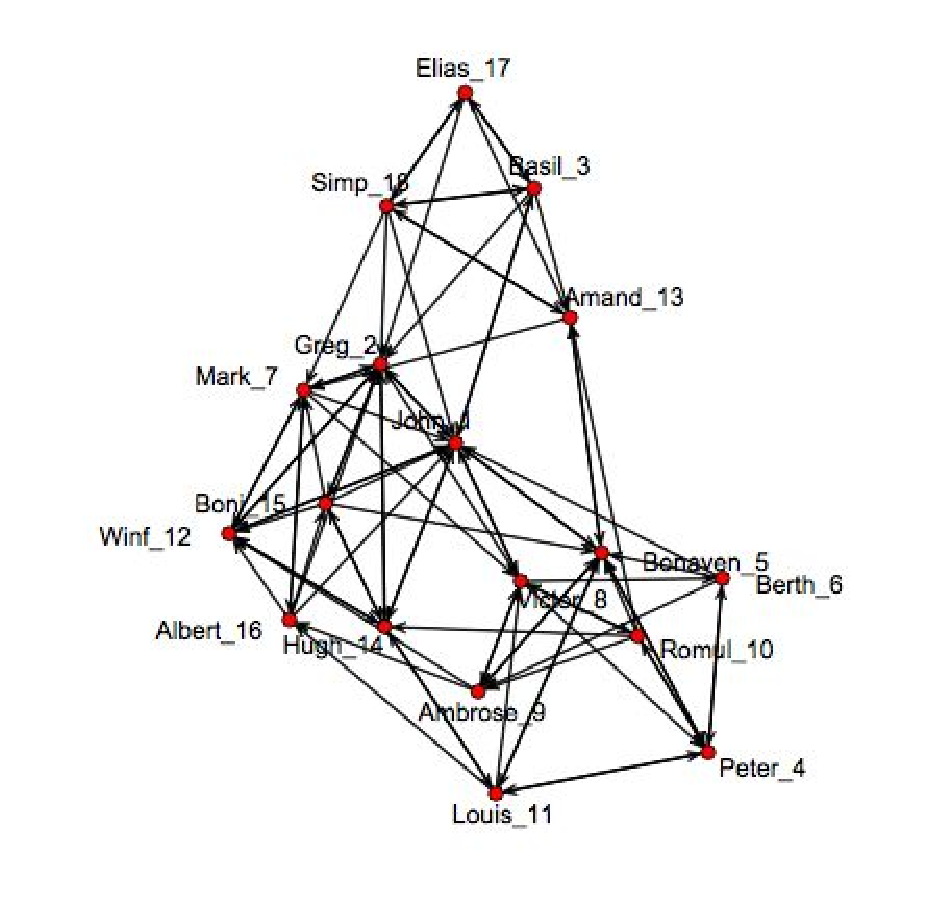
\includegraphics[height=2.8in]{samplike}
\caption{Sampson's (1969) monastery affinity network among 18 monks.} 
\end{center} 
\end{figure}
}
\frame
{
  \frametitle{and... }

\begin{figure}
\begin{center} 
\includegraphics[height=2.7in]{florentine}
\caption{Padgett's (1994) Florentine marriage network among 16 Florentine families around 1430.} 
\end{center} 
\end{figure}
}
\frame
{
  \frametitle{and... }
\begin{figure}
\begin{center} 
\includegraphics[height=2.7in]{fmh-gradesex2}
\caption{National Longitudinal Study of Adolescent Health friendship network of 1,461 students in grades 7 -- 12 without isolates.  Squares=Boys, Circles=Girls.} 
\end{center} 
\label{fmh} 
\end{figure}
}
\frame
{
  \frametitle{and...}

\begin{figure}
\begin{center} 
\includegraphics[height=2.7in]{ecoli}
\caption{E. Coli transcriptional regulation network of Shen-Orr et al. (2002).  
Nodes are operons, $i \to j$ indicates that $i$ encodes transcription factor that regulates $j$.} 
\end{center} 
\end{figure}
}

\frame
{
\frametitle{Why networks?}
Networks are a conduit for \emph{flow}.  
\vspace{2mm}

Flow can be:
\begin{itemize}
\item friendship
\item diseases
\item needle-sharing
\item money
\item data
\item airplanes
\item commodities
\item ideas
\item advice 
\item association (among terrorists)
\item binding (between proteins)
\end{itemize}
\vspace{2mm}

\textbf{Goal of a network model: explain the mechanism of this flow.} 
}

%%%%%%%%%%%%%%%%%%%%%%%%%%%%%%%%%%%%%%%%%%%%%%%%%%%%%%%%%%%%%
\section{Modeling}
\frame
{
\frametitle{A network, mathematically}
A social network is a collection of \emph{actors} and the \emph{relations}, or \emph{ties}, between each pair of actors.  

We can represent a network with $n$ actors as an $n \times n$ matrix $Y$, where each entry
\begin{align*}
	Y_{ij} =
	\begin{cases} 	1 \quad \text{if a relation exists from actor $i$ to actor $j$}\\
					0 \quad \text{otherwise}
	\end{cases}
\end{align*}

The Sampson monastery network (directed), in matrix form:
{\tiny
\begin{table}[ht]
\begin{center}
\begin{tabular}{rrrrrrrrrrrrrrrrrr}
  \hline
0 & 1 & 1 & 0 & 1 & 0 & 1 & 0 & 0 & 0 & 1 & 0 & 0 & 0 & 1 & 0 & 0 & 0 \\ 
0 & 0 & 1 & 0 & 1 & 1 & 0 & 0 & 1 & 0 & 0 & 0 & 0 & 0 & 1 & 0 & 0 & 0 \\ 
0 & 1 & 0 & 0 & 0 & 0 & 1 & 1 & 0 & 0 & 0 & 0 & 0 & 1 & 0 & 0 & 0 & 0 \\ 
0 & 1 & 1 & 0 & 1 & 0 & 0 & 0 & 1 & 0 & 0 & 0 & 0 & 0 & 0 & 0 & 0 & 0 \\ 
1 & 1 & 0 & 1 & 0 & 1 & 0 & 0 & 0 & 0 & 0 & 0 & 0 & 0 & 0 & 0 & 0 & 0 \\ 
0 & 1 & 0 & 0 & 1 & 0 & 1 & 0 & 0 & 0 & 1 & 0 & 0 & 1 & 0 & 0 & 0 & 0 \\ 
1 & 0 & 1 & 1 & 1 & 0 & 0 & 0 & 1 & 1 & 0 & 0 & 0 & 0 & 0 & 0 & 0 & 0 \\ 
0 & 0 & 0 & 0 & 0 & 0 & 0 & 0 & 1 & 1 & 1 & 0 & 1 & 0 & 0 & 0 & 0 & 0 \\ 
0 & 1 & 0 & 0 & 0 & 0 & 1 & 1 & 0 & 1 & 1 & 0 & 0 & 0 & 0 & 1 & 0 & 0 \\ 
0 & 0 & 0 & 0 & 0 & 0 & 0 & 1 & 1 & 0 & 1 & 1 & 1 & 0 & 0 & 0 & 0 & 0 \\ 
0 & 0 & 0 & 0 & 0 & 1 & 0 & 1 & 1 & 1 & 0 & 1 & 0 & 0 & 0 & 0 & 0 & 0 \\ 
0 & 1 & 0 & 0 & 0 & 0 & 0 & 1 & 1 & 1 & 1 & 0 & 1 & 0 & 0 & 0 & 0 & 0 \\ 
0 & 0 & 0 & 0 & 0 & 0 & 1 & 1 & 1 & 1 & 0 & 0 & 0 & 1 & 0 & 0 & 0 & 0 \\ 
0 & 0 & 0 & 0 & 0 & 0 & 0 & 1 & 1 & 1 & 0 & 1 & 1 & 0 & 0 & 0 & 0 & 0 \\ 
0 & 1 & 0 & 0 & 0 & 0 & 0 & 0 & 0 & 0 & 0 & 0 & 1 & 0 & 0 & 0 & 0 & 1 \\ 
0 & 0 & 0 & 0 & 0 & 0 & 0 & 0 & 1 & 1 & 0 & 0 & 0 & 0 & 1 & 0 & 1 & 1 \\ 
0 & 0 & 0 & 0 & 0 & 0 & 0 & 0 & 0 & 1 & 0 & 0 & 0 & 0 & 1 & 1 & 0 & 1 \\ 
0 & 0 & 0 & 0 & 0 & 0 & 0 & 0 & 1 & 1 & 0 & 0 & 1 & 0 & 1 & 1 & 1 & 0 \\ 
   \hline
\end{tabular}
\end{center}
\end{table}}
}
\frame
{
\frametitle{01101010001 ...}
Take this matrix and represent element with 0 as white, 1 as Black.
%\pause
\begin{figure}
\begin{center} 
\includegraphics[height=1.5in]{samplike-matrix}
%\caption{} 
\end{center} 
\end{figure}
%\pause
\textbf{$Y_{ij}$ are not in general independent.  This dependence is at the core of the ``network perspective''.}
\vspace{1mm}

%\pause
Statistical inference: determine what effects are important in shaping 
global structure of relations.  
\vspace{1mm}

``Predictors" may be actor specific attributes: grade or gender.
But also want to include salient relational structures that capture dependence.
}

\frame
{
\frametitle{A network model}

Writing down an expression for a network model is easy.  

Exponential-family Random Graph Models (ERGM) have a log likelihood
\begin{align*}% \label{E:loglike}
	\ell( \eta) = \inner{\eta, g(\yobs)} - c(\eta)
\end{align*}
where
\begin{align*}
	c(\eta) = \log \sum_{y \in \YY} e^{\inner{\eta, g(y)}}.
\end{align*}

The natural statistic $g(y)$ is a vector of \emph{network statistics} of interest.  Some examples:
\begin{itemize}
	\item number of edges, $\sum_{i<j} Y_{ij}$
	\item number of triangles, $\sum_{i < j < k} Y_{ij}Y_{jk}Y_{ki}$
\end{itemize}
So, in this case,
\begin{align*}
	g(y) = \left( \sum_{i<j} Y_{ij}, 
					\sum_{i < j < k} Y_{ij}Y_{jk}Y_{ki} \right ).
\end{align*}


}


\frame
{
\frametitle{Number of graphs in $\YY$}
\begin{table}[h!] 
\caption{Sample space size for undirected networks with different number of 
actors.}

\begin{tabular}{ccl} 
\hline 
Nodes & Possible Edges & Total Graphs \\ [1ex]
\hline
5 & ${5 \choose 2} = 10$ & $2^{10} = 1024$ \\ [1ex]
6 & ${6 \choose 2} = 15$ & $2^{15} = 32,768$ \\ [1ex]
7 & ${7 \choose 2} = 21$ & $2^{21} = 2,097,152$ \\ [1ex]
8 & ${8 \choose 2} = 28$ & $2^{28} = 268,435,456$ \\ [1ex]
9 & ${9 \choose 2} = 36$ & $2^{36} = 68,719,476,736$ \\ [1ex]
10 & ${10 \choose 2} = 45$ & $2^{45} = 3.518437\times10^{13}$ \\ [1ex]
\hline 
\end{tabular} \label{T:number graphs}
\end{table}

So, the sum in $c(\eta)$ is over an astronomical number of terms for 
even moderate sized networks.
\vspace{2mm}

\textbf{Implication: don't evaluate the log likelihood function.}
}

%%%%%%%%%%%%%%%%%%%%%%%%%%%%%%%%%%%%%%%%%%%%%%%%%%%%%%%%%%%%%
\section{Parameter estimation}
\frame
{
\frametitle{Calibrating}
What is the value for $\eta$ such that the model assigns the highest probability to the observed data?
\vspace{2mm}

Maximum likelihood estimator (MLE)!
\vspace{2mm}

great.
\vspace{2mm}

But how do you find this value that maximizes the likelihood if \emph{you can't evaluate the likelihood?}
\vspace{2mm}

Thanks for nothing.
}

\frame
{
\frametitle{Methods that are out there}
\begin{center} 
\includegraphics[height=3in]{mck-before.png}
%\caption{Adolescent Health.} 
\end{center} 
}
%\frame
%{
%\frametitle{Methods that are out there}
%\begin{figure}
%\begin{center} 
%\includegraphics[height=3in]{mck-after.png}
%%\caption{Adolescent Health.} 
%\end{center} 
%\end{figure}
%}
%%%%%%%%%%%%%%%%%%%%%%%%%%%%%%%%%%%%%%%%%%%%%%%%%%%%%%%%%%%%%%
\section{Long range algorithm (part I)}
\frame
{
\frametitle{Designing an algorithm: wish list}

Our algorithm should
\begin{itemize}
\item Converge to the MLE $\etaMLE$, if it exists.
\item Work from \emph{any} starting point $\eta_0$.
\item No trial-and-error calibration.
\end{itemize}
\vspace{2mm}

Some implications of the above:
\begin{itemize}
\item Don't evaluate log likelihood function $\ell( \eta)$
\item Don't use second derivative of log likelihood $\nabla^2 \ell( \eta)$
\begin{itemize}
	\item Can be expensive to compute
	\item Not informative when $\eta_0$ is far from solution---may be near-singular
\end{itemize}
\end{itemize}
}

\frame
{
\frametitle{So what \emph{do} we have??}
{\textbf{We have the \emph{gradient},} $\boldsymbol{\nabla \ell(\eta)}$.}
\vspace*{2mm}

By a nice property of exponential families,
\begin{align*}
	\nabla \ell( \eta ) = g(y_{obs}) - \E_{\eta} g(Y).
\end{align*}


Even when $E_\eta g(Y)$ cannot be calculated exactly, it can be well approximated by
\begin{align*}
E_\eta g(Y) \approx \frac{1}{m}\sum_{i = 1}^m g(Y_i),
\end{align*}
where $Y_1$, $\ldots$, $Y_m$ are an MCMC sample from distribution with parameter $\eta$.
\vspace*{4mm}

%\pause
We need to find a way to use the gradient to: 
\vspace*{2mm}
\begin{itemize}
\item Direct the search  (Determine $p_k$)
\vspace*{2mm}

\item Ensure that adequate progress is made in each iteration  (Pick $\alpha_k$)
\vspace*{2mm}

\item Inform us when the MLE is obtained  ($\nabla \ell(\eta) = 0$)
\end{itemize}

}

\frame
{
\frametitle{Framework for our algorithm}
Use simple iterated estimates
\begin{align*}
	\eta_{k+1} = \eta_k + \alpha_k p_k
\end{align*}
where $\alpha_k$ is a \textbf{step size} and  $p_k$ is a \textbf{search direction} that
is restricted to be an \emph{ascent direction} of the log likelihood.
\vspace{2mm}

Taking positive step sizes $\alpha_k$ in an ascent direction $p_k$ gets us ``progress" up the log 
likelihood surface in the direction of $p_k$, but does not assure us 
``\emph{sufficient} progress".
\vspace{2mm}

We need a condition that guarantees good step sizes $\alpha_k$.
}


\frame
{
  \frametitle{Curvature condition}
Find an $\alpha_k$ that satisfies
\begin{align*}
	 0 & \leq \nabla \ell( \eta_k + \alpha_k p_k)^T p_k \leq c \nabla \ell(\eta_k)^T 
p_k
\end{align*}
\begin{figure}[h]
\centering
    \scalebox{.25}{\input{Figures/alphamax.pdf_t}}
	\caption{Acceptable region for step size $\alpha_k$ along a search direction $p_k$.}
\label{F:alpha_region}
\end{figure}
}



\frame
{
\frametitle{Search Algorithm}
\setbeamercovered{transparent}
\small

Get an initial value, $\eta_0$.\\ 
Set $k=0$. \\
Set $p_0 = \nabla \ell( \eta_0)$, the direction of steepest ascent. \\
\vspace*{2mm}

\uncover<2->{
\textbf{while}  $\parallel \nabla \ell( \eta_k) \parallel > \epsilon$ \\ 
\vspace*{1mm}

\uncover<3->{
\hspace*{4mm} \textbf{Find} \alert{$\alpha_k$} that satisfies the \textbf{curvature condition}
\begin{align*}
	 0 & \leq \nabla \ell( \eta_k + \alert{\alpha_k} p_k)^T p_k \leq c \nabla \ell(\eta_k)^T p_k
\end{align*}
\hspace*{4mm} \indent for some fixed $0 < c < 1$.  
\vspace*{1mm}
} 

\uncover<4->{
\hspace*{4mm} $\eta_{k+1} = \eta_k + \alert{\alpha_k} p_k$\\
\vspace*{1mm}
\hspace*{4mm} $\nabla \ell( \eta_{k+1}) = g( y _{obs}) - \E_{\eta_{k+1}}g(Y)$\\
\vspace*{2mm}
} 

\uncover<5->{
\hspace*{4mm} \indent \textbf{Find} \alert{$p_{k+1}$}
, which must be an ascent direction. \\
}

\uncover<6->{
\hspace*{4mm} \indent $k = k + 1$  \\
}

\textbf{end(while)}
}  
}



\frame
{
\frametitle{Results}
{\small
\begin{theorem}[Exponential family zero gradient attainment] \label{Thm:log like max}
Consider any line search of the form 
\begin{align}
	\eta_{k+1} &= \eta_k + \alpha_k p_k \label{E:eta_update}
\end{align}
used to minimize the negative log likelihood function $-\ell(\cdot)$ of a regular 
exponential family on a finite sample space, where the search direction $p_k$ 
is a descent direction.
%such that the angle $\theta_k$ between the search direction $p_k$ and steepest descent 
%direction $-\nabla \ell(\eta_k)$ is 
%restricted to be less than 90 degrees by
%\begin{align*}
%\cos \theta_k \geq \delta > 0
%\end{align*}
% for some fixed $\delta > 0$.  

Then it is possible to find a step length $\alpha_k$ 
that satisfies the \emph{curvature condition}
\begin{align}
	0 \leq \nabla \ell( \eta_k + \alpha_k p_k)^T p_k  \leq c \nabla \ell(\eta_k)^T p_k  
\label{E:Wolfe-ll}
\end{align}
for some fixed $0 < c < 1$.

Furthermore, repeated iterations of \eqref{E:eta_update} along a descent direction 
satisfying \eqref{E:Wolfe-ll} will produce a sequence, $\eta_1, \eta_2, \ldots$ such 
that
\begin{align*}
	\lim_{k \to \infty} \lVert \nabla \ell(\eta_k) \rVert = 0.
\end{align*}
\end{theorem}
}
}

\frame
{
\frametitle{MLE attainment}
Previous theorem gives us using our algorithm gets us 
$\lVert \nabla \ell(\eta_k) \rVert \to 0$.  

A little more work gets us that 
this is the same thing as finding the MLE $\etaMLE$.

\begin{theorem}[MLE convergence] \label{Thm:Line Search works}
For a regular exponential family with minimal representation where the MLE exists, the 
line search described in 
Theorem~\ref{Thm:log like max} can be applied to the negative log likelihood function 
$-\ell(\eta)$ so that a search 
starting at any $\eta_0 \in \Xi$ will converge to the MLE of $\eta$.
\end{theorem}

}

%%%%%%%%%%%%%%%%%%%%%%%%%%%%%%%%%%%%%%%%%%%%%%%%%%%%%%%%%%%%%
\section{Examples}
\frame
{
  \frametitle{Toy example: Monks}  
\begin{columns}[t]
\begin{column}[T]{0.3\textwidth}
%\includegraphics[height=1.5in]{g9-basic}
%\pgfputat{\pgfxy(0,0)}{\pgfbox[left,top]{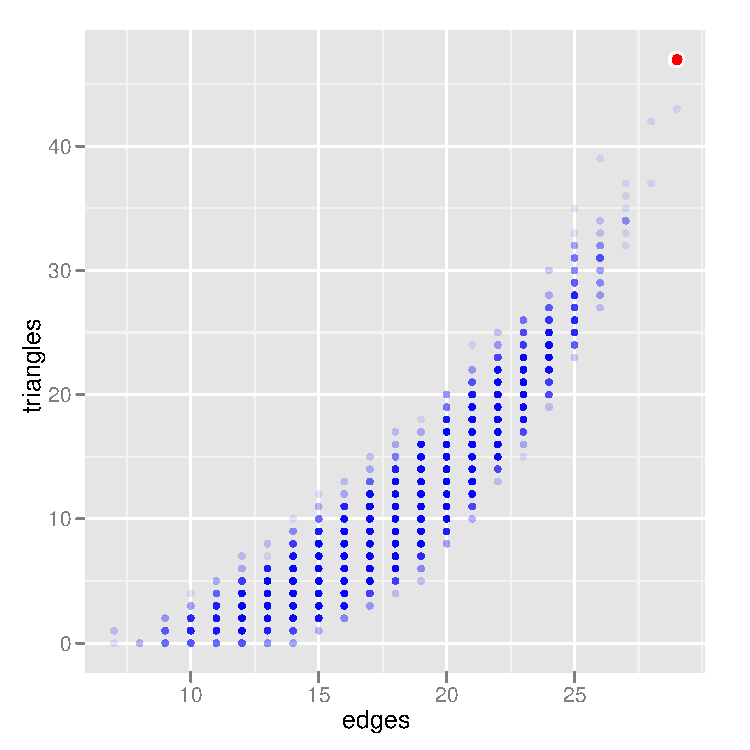
\includegraphics[width=\textwidth]{MCsample-bare} }}
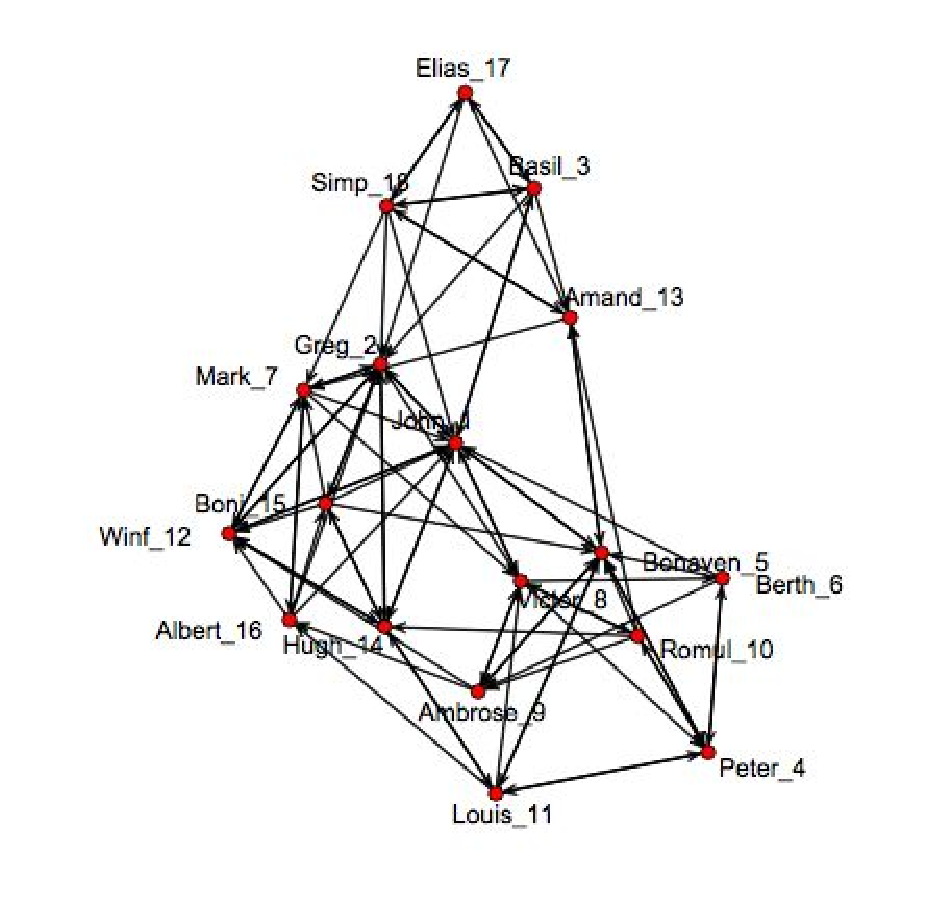
\includegraphics[width=1.5in]{samplike}
\end{column}

\begin{column}[r]{0.7\textwidth}
Use a simple model with only edges.  For this model, $\etaMLE$ can be 
determined analytically,
\begin{align*}
	\etaMLE = -0.9072.
\end{align*}

MCMC-MLE may struggles to converge when
starting value $\eta_0$ is far from $\etaMLE$;

starting from $\eta_0 = 1$ took
10 iterations to converge (default in \texttt{ergm} package is three).
\end{column}
\end{columns}

We ran our algorithm starting at same $\eta_0=1$.  Our algorithm converged
after 21 iterations with 5 parameter updates.
{\footnotesize
\begin{table}
\begin{center}
\begin{tabular}{rrrrrrlrr}
  \hline
    &  &  &  & \multicolumn{1}{c}{inner}\\
  \multicolumn{1}{c}{$k$} & 
  \multicolumn{1}{c}{$\eta_k$} &
  \multicolumn{1}{c}{$\lVert \nabla \ell(\eta_k) \rVert$} &
  \multicolumn{1}{c}{$\alpha_k$} &
  \multicolumn{1}{c}{loop }\\
    &  &  &  & \multicolumn{1}{c}{count}\\
  \hline
   0 &  $1.0000$ & 135.64 &  0.012 & 8\\
   1 & $-0.6649$ & 15.99  &  0.014 & 2 \\
   2 & $-0.8817$ & 1.57   &  0.014 & 3 \\
   3 & $-0.9043$ & 0.22   &  0.012 & 8 \\
   4 & $-0.9069$ & 0.03   &  &  \\
   \hline
\end{tabular} \label{T:Sampson redo}
\end{center}
\end{table}}
}

\frame
{
  \frametitle{Example: large friendship network}  
\begin{columns}[t]
\begin{column}[T]{0.3\textwidth}
%\includegraphics[height=1.5in]{g9-basic}
%\pgfputat{\pgfxy(0,0)}{\pgfbox[left,top]{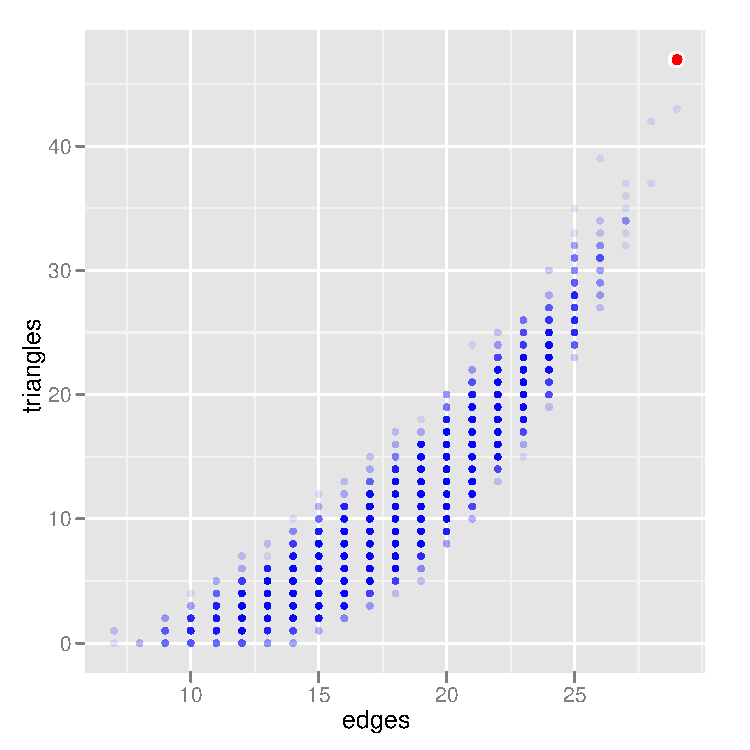
\includegraphics[width=\textwidth]{MCsample-bare} }}
\includegraphics[width=1.45in]{fmh-gradesex2}
\end{column}

\begin{column}[T]{0.7\textwidth}
Fit with a more realistic model that includes terms for actor 
specific attributes in addition to network structures.  
%\vspace{1mm}

Actor specific attributes: Grade, Race, Sex.
\vspace{2mm}

Network structures: edges and geometrically weighted edgewise shared partners (GWESP)
\vspace{2mm}

Run our algorithm starting at $(0,0,0,0,0)$, compare to MCMC-MLE (starting at a value very close to MLE).
\end{column}
\end{columns}
\vspace{1mm}

Stopped our algorithm after 40 updates.
\begin{table}
\begin{center} 
%\caption[Comparison of MLEs for $\eta$ for MCMC-MLE and our algorithm for Faux Magnolia High example]{Comparison of MLEs for $\eta$ for MCMC-MLE and our algorithm for Faux Magnolia High example.  MCMC-MLE is the default algorithm
%in \texttt{ergm}, and is run here through 5 iterations starting
%at the MPLE ($\etaMLE$ below).
%Our algorithm is run for 40 steps ($\hat{\eta}_{\textrm{Steep}}$ below),
%starting from $(0,0,0,0,0)$.\\
%}
\begin{tabular}{rrrrrr}
  \hline
 & edges & Grade & Race & Sex & GWESP \\ 
  \hline
$\etaMLE$ & -9.790 & 2.755 & 0.906 & 0.780 & 1.813 \\ 
$\hat{\eta}_{\textrm{Steep}}$ & -9.879 & 2.810 & 0.942 & 0.786 & 1.809 \\ 
   \hline
\end{tabular}\label{T:FauxMagnolia}
\end{center}
\end{table}
}







%%%%%%%%%%%%%%%%%%%%%%%%%%%%%%%%%%%%%%%%%%%%%%%%%%%%%%%%%%%%%
\section{non-Existent MLEs}
\frame
{
  \frametitle{Geyer, 2009}  

In 2009, Geyer woofed$^1$ about a way to handle non-existent MLEs in the case of generalized linear models.
\vspace{2mm}

Log likelihood is a strictly concave function.  

For the MLE not to exist, there must be a direction $\delta$ for which
$\ell(\eta + s\delta)$ is strictly increasing in $s$.

Such a $\delta$ is called a \textbf{direction of recession (DOR)}, 
and exists if and only if the
observed data $g(\yobs)$ lies on the relative boundary of the \textbf{convex support} of the model.
\vspace{2mm}

So what to do?

The MLE is ``off at infinity" in the direction of $\delta$.

But Geyer showed that it is possible to give a measure of how parameter $\eta$ is to infinity using one-sided confidence intervals:
\begin{align*}
	[\hat{\eta}_L, +\infty)
\end{align*}

\vspace{0.2in}
\footnotesize{$^1$Actually, Geyer had been woofing about MLE existence since at least as early as 1990.}
}

\frame
{
  \frametitle{Conditions for non-existent MLE---graphically}  
The \textbf{convex support} $C$ is the smallest closed convex set that contains the natural statistics.
%\vspace{2mm}

\begin{columns}[T]
\begin{column}[T]{0.45\textwidth}
\vspace{4mm}

{\small
Example: 9-node undirected network with edge and triangle statistics.
\begin{itemize}
\item 69 billion possible graphs in $\YY$.
\item Only 444 possible edge-triangle combinations.
\item $C$ is a 6-sided polytope.
\end{itemize}

\textbf{MLE exists if and only if
$g(\yobs)$ is in interior of $C$.}
}
\end{column}
\begin{column}[T]{0.55\textwidth}
\begin{figure}[h]
\centering
\includegraphics[height=2.6in]{g9-hull}
%\caption{Convex support for 9-node undirected network model with edge and triangle
%statistics.}
%\label{F:g9-hull}
\end{figure}
\end{column}
\end{columns}
}

\frame
{
  \frametitle{Condition for non-existent MLE---theoretically}  
\begin{theorem}[Extension of Theorem 4 (Geyer, 2009)]
For a full exponential family with with log likelihood \eqref{E:loglike}, convex support $C$, and observed data $\yobs$, the following are equivalent:
\begin{enumerate}
\item the MLE exists.
\item Every direction of recession is direction of constancy.
\item $N_C(g(\yobs))$ is a vector subspace.
\item $T_C(g(\yobs))$ is a vector subspace.
\item $g(\yobs) \in \rint C$.
\end{enumerate}
\end{theorem}
}

\frame
{
	\frametitle{Observed data is on boundary.  So then what??}

Define a hyperplane $H$, orthogonal to $\delta$, a direction of recession.
\begin{figure}[h]
\centering
\includegraphics[height=2.4in]{g9-H.png}
%\caption{Convex support for 9-node undirected network model with edge and triangle statistics.}
%\label{F:g9-hull}
\end{figure}
Then as $s \to +\infty$,
\begin{align*}
		P_{\eta + s \delta}( g(Y) \in H) \to 1.
\end{align*}
}

\frame
{
  \frametitle{Limiting conditional model (LCM)}  
	The limiting distribution, called the \textbf{limiting conditional model (LCM)}, is another exponential family where
	\begin{itemize}
		\item the convex support is the convex hull of $g(\YY) \cap H$.
		\item $P_{\eta + s \delta}( Y = y) \to P_{\eta}( Y =y \mid g(Y) \in H)$.
		\item $\ell(\eta) < \ell_{LCM}(\eta)$, where $\ell_{LCM}(\eta)$ is the log likelihood of the LCM.
		\item the MLE, $\etaLCM$, is guaranteed exists.
	\end{itemize}
}
\frame
{
  \frametitle{Measuring closeness to infinity}  
So,
\begin{align*}
	\lim_{s \to +\infty} \ell(\etaLCM + s\delta) = \sup_{\RR^d} \ell(\eta).
\end{align*}	

MLE for original model: off at $+\infty$.

Now, some more detail: it is $\etaLCM$ sent to infinity in direction of $\delta$.
\vspace{2mm}

Can we say anything about how close $\eta$ is to infinity?  

Find unique $s$, call it $\hat{s}$, such that
\begin{align*}
		P_{\etaLCM + s \delta}( g(Y) \in H) = \alpha.
\end{align*}
Then $[ \hat{s}, +\infty)$ is a $1- \alpha$ confidence interval for the parameter $s$, and
\begin{align*}
[ \etaLCM + \hat{s} \delta, + \infty)
\end{align*}
gives a $1 - \alpha$ confidence region for the parameter $\etaLCM + \hat{s} \delta$.
}

%\frame
%{
%  \frametitle{Previous work}  
%
%\begin{columns}[t]
%%
%\begin{column}[2in]
%Handcock (2003), Rinaldo, Fienberg, and Zhou (2009).
%\end{column}
%
%\begin{column}[4in]
%\begin{figure}[h]
%\centering
%\includegraphics[height=2.6in]{g9-hull}
%\caption{Convex support for 9-node network model with edge and triangle
%statistics.}
%%\label{F:g9-hull}
%\end{figure}
%\end{column}
%\end{columns}
%}
\frame
{
  \frametitle{Previous work}  
Handcock (2003), Rinaldo, Fienberg, and Zhou (2009) studied 7 and 9-node undirected networks
with two statistics.
\begin{itemize}
	\item Confirmed condition for relative location of $g(\yobs)$ for MLE to not exist.  
	%That is, found face of $C$ in which $g(\yobs)$ lies in relative interior.
	\item Identified cones that bound DORs.% (normal cones of $C$ at $g(\yobs)$).
\end{itemize}

Authors use full knowledge of convex support of model $C$ to determine above.

\begin{columns}[]
\begin{column}[T]{0.4\textwidth}
\includegraphics[width=1.9in]{g9-basic}
\end{column}
\begin{column}[T]{0.6\textwidth}
In particular, H-representation of $C$:
\begin{align*}
	Ax \leq b.
\end{align*}
Easy to check if a point is in exterior, interior, or boundary of hull.

\end{column}
\end{columns}
\textbf{But in a real problem, we don't have this!  So, no general method suggested.}

}

%%%%%%%%%%%%%%%%%%%%%%%%%%%%%%%%%%%%%%%%%%%%%%%%%%%%%%%%%%%%%
\section{Algorithm extended}
\frame
{
\frametitle{What do we have?}
MCMC samples from distribution with parameter $\eta_k$.  

And here, we're trying to do more: find $\etaLCM$ and 
a GDOR $\delta$.
\vspace{1ex}

\begin{columns}[t]
\begin{column}[T]{0.4\textwidth}
%\includegraphics[height=1.5in]{g9-basic}
%\pgfputat{\pgfxy(0,0)}{\pgfbox[left,top]{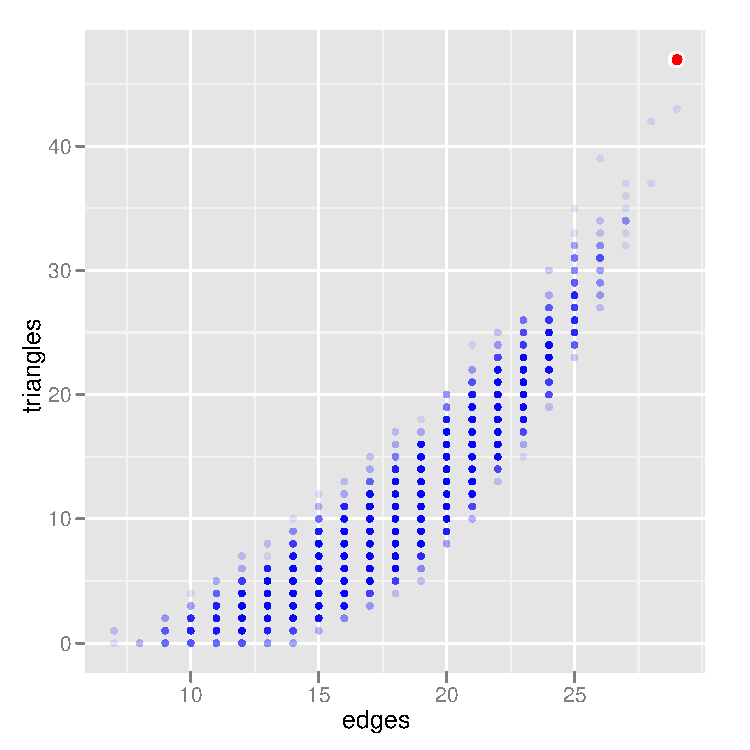
\includegraphics[width=\textwidth]{MCsample-bare} }}
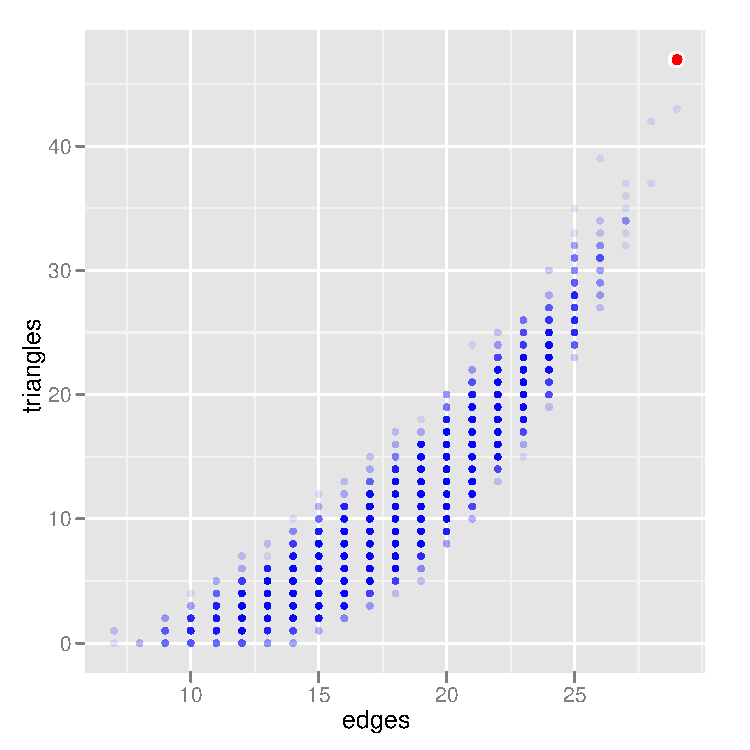
\includegraphics[width=2in]{MCsample-bare}
\end{column}

\begin{column}[r]{0.6\textwidth}
\begin{itemize}
\item But that's all we needed to find the MLE before! 
%\vspace{1mm}


\item Iterated sampling from distribution with parameter $\eta_k$ until $\nabla \ell(\eta_k) = 0$.

Or alternatively, until
\begin{align*}
	\E_{\eta_k} g(Y) = g(\yobs).
\end{align*}

\end{itemize}
\end{column}
\end{columns}
}

\frame
{
\frametitle{Case: MLE exists}  
\begin{figure}[h]
\centering
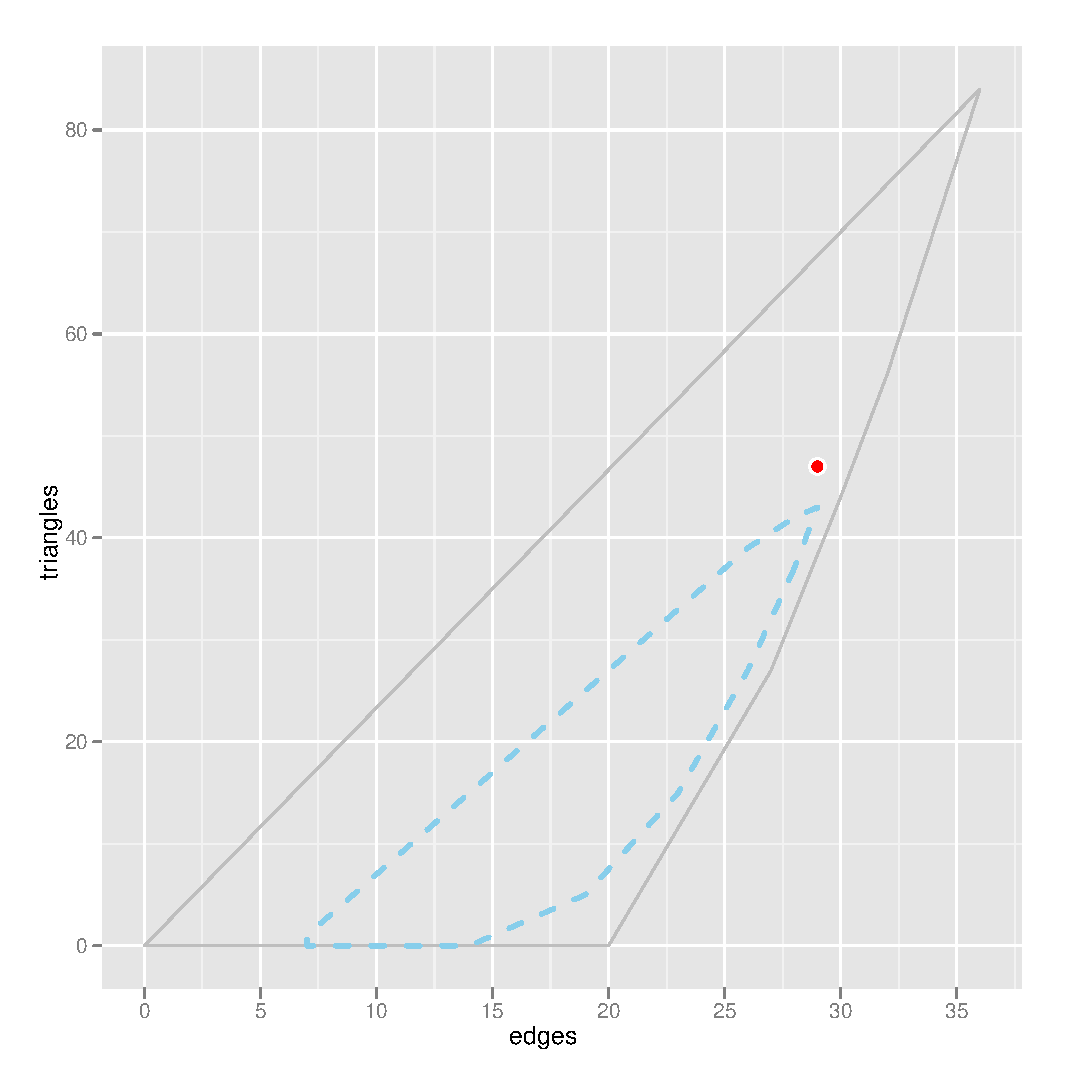
\includegraphics[height=2.2in]{MCsample-far}
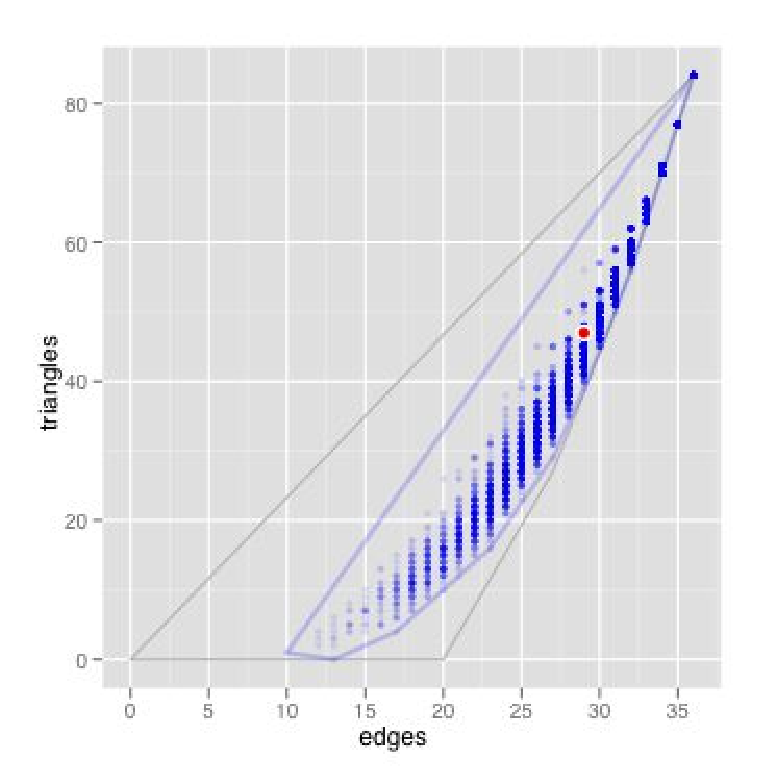
\includegraphics[height=2.2in]{MCsample-MLE}
\caption{MCMC samples from distributions with $\eta = (0,0)$ (left), and $\eta=\etaMLE$ (right).}
\label{F:MCsample-MLE exists}
\end{figure}
%MCMC samples from distributions with $\eta = (0,0)$ (left), and $\eta=\etaMLE$ (right).
}


\frame
{
\frametitle{Extend our algorithm}  
\textbf{Idea}: Use MCMC samplers to explore space of natural statistics and
determine geometry of convex support $C$.
\vspace{2mm}

\includegraphics[width=2.2in]{minesweeper}
\vspace{2mm}

Our algorithm climbs up log likelihood.  So we know that cloud of points will move towards $g(\yobs)$.
\vspace{2mm}

Need to find a way to determine if
\begin{enumerate}
\item $g(\yobs)$ is on the boundary of our sample hull.
\item If so, on what face of our sample hull does it lie?
\item Is the boundary of the sample hull also the boundary of $C$?
\end{enumerate}
}

\frame
{
\frametitle{Case: MLE does not exists}  
\begin{figure}[h]
\centering
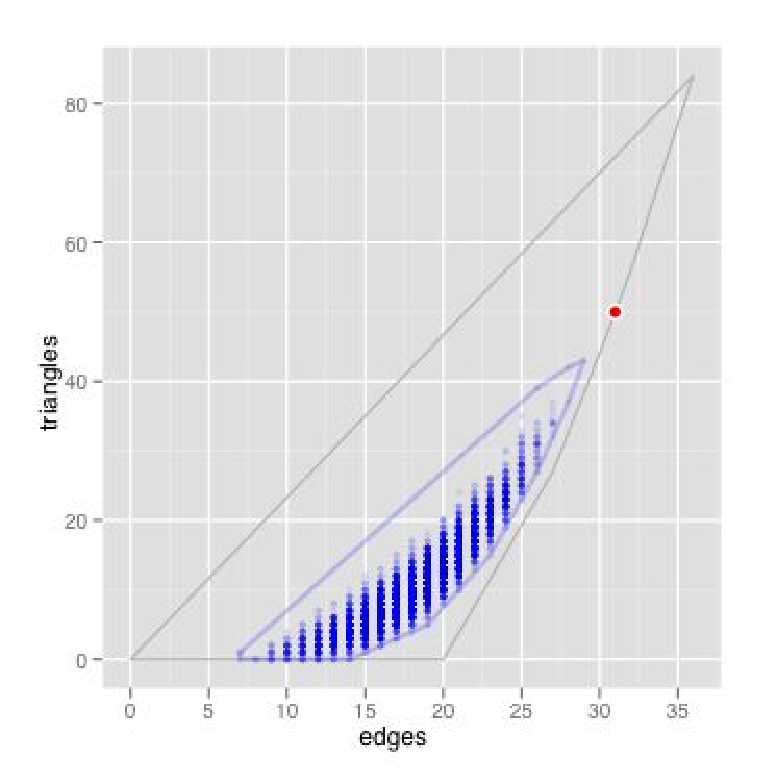
\includegraphics[height=2.2in]{MCsample-boundary}
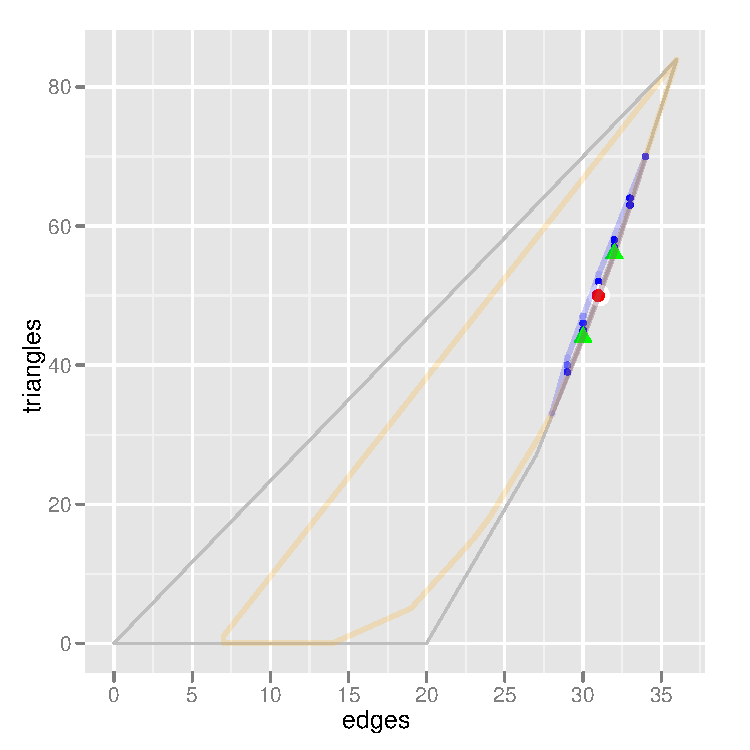
\includegraphics[height=2.2in]{MCsample-77face}
\caption{MCMC samples from distributions with $\eta = (0,0)$ (left), and $\eta=$ (right).}
\label{F:MCsample-MLE nonexistent}
\end{figure}
}

\frame
{
\frametitle{\texttt{rcdd} to the rescue}  
\begin{columns}[T]
\begin{column}[T]{0.25\textwidth}
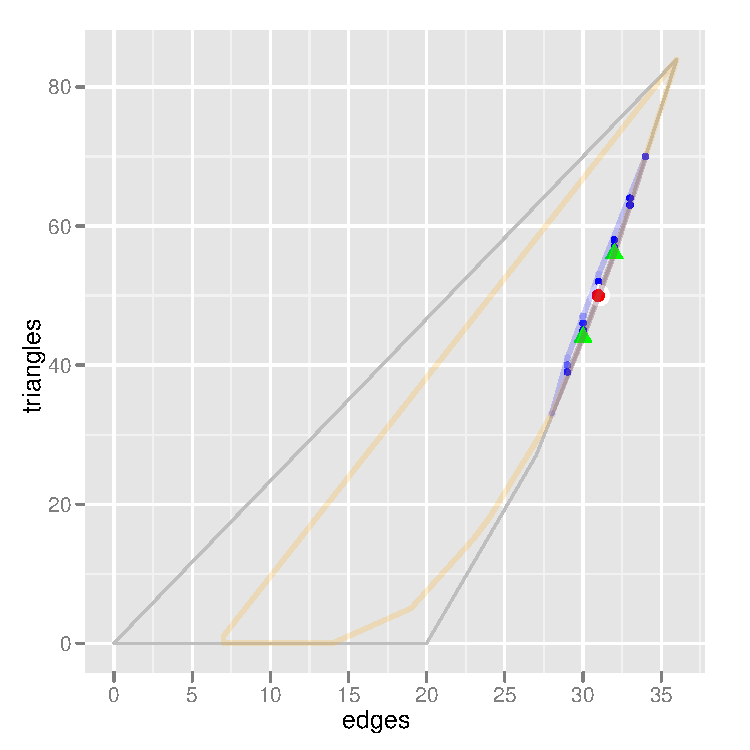
\includegraphics[height=2.5in,trim=3.5in 2in 0.15in 0.05in,clip=true]{MCsample-77face} % l b r t
\end{column}
\begin{column}[T]{0.75		\textwidth}
These are problems in \emph{computational geometry}.  Fortunately, 
the \texttt{rcdd} package (Geyer and Meeden, 2009) has the linear programming 
tools we need to answer these questions.
\vspace{2mm}

\begin{enumerate}
\item $g(\yobs) \notin$ sample hull.  Look for a strongly separating hyperplane.
\item Find face $F$ on which $g(\yobs)$ lies in relative interior.
\item Find a GDOR $\delta$ to $F$.
\end{enumerate}
Can do all these while without calculating H-representations of hulls.


One thing it does not do: tell us if $F$ of the hull of our samples is also
on the boundary of $C$.  
\vspace{2mm}

Our approach: if $>60\%$ of samples land on what we determined is a face, then it is on the boundary.
\vspace{2mm}

Here, 77\% of the samples fall on three points (including $g(\yobs)$) that define a face, also on the boundary of $C$.
\end{column}
\end{columns}
}

\frame
{
\frametitle{Then what?}  
Oh right, we wanted one-sided CIs for $\eta$.

We we have found is a GDOR $\delta$ and a face $F$ in which $g(\yobs)$ lies
in the relative interior.

Theorem says that $F$ is the support for the LCM.  Since MLE for LCM is guaranteed to exist, our algorithm can be applied as before to find it.

Find $\etaLCM$, the MLE in the limiting conditional model.

Finally, one-sided CI.
Find unique $s$, call it $\hat{s}$, such that
\begin{align*}
		P_{\etaLCM + s \delta}( g(Y) \in H) = \alpha.
\end{align*}
Then $[ \hat{s}, +\infty)$ is a $1- \alpha$ confidence interval for the parameter $s$, and
\begin{align*}
[ \etaLCM + \hat{s} \delta, + \infty)
\end{align*}

In this example where $g(\yobs) = (31,50)$, 
\begin{align*}
	\etaLCM = (126.8, -21.1)\\
	\delta = (6,-1)
\end{align*}
and a one-sided 95\% CI yields
\begin{align*}
	[9.145, +\infty) \\
	(-\infty, -1.500].
\end{align*}


}

%\frame
%{
%\frametitle{Case: MLE exists, but observed data close to boundary}  
%\begin{figure}[h]
%\centering
%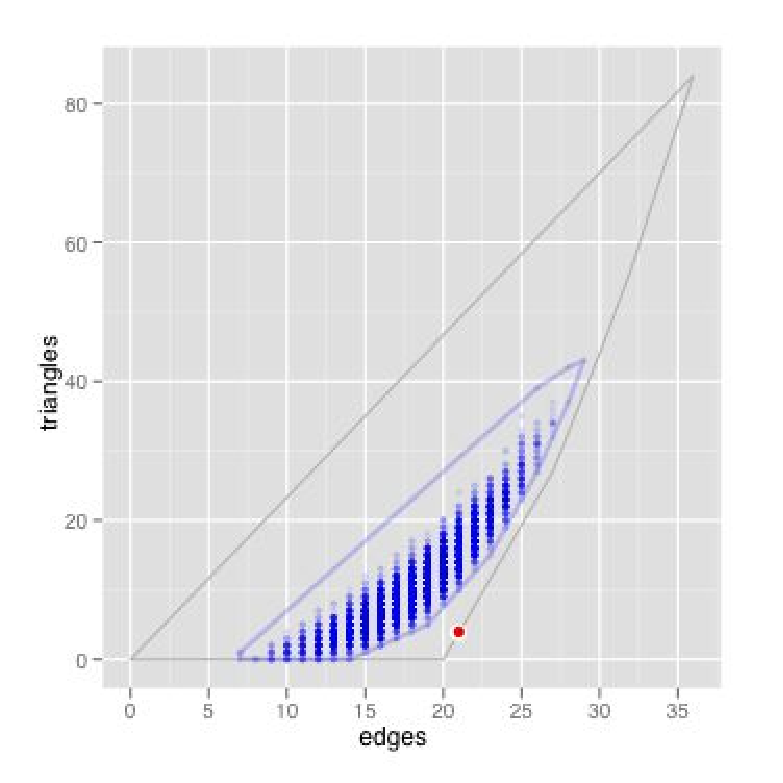
\includegraphics[height=2.5in]{MCsample-problem}
%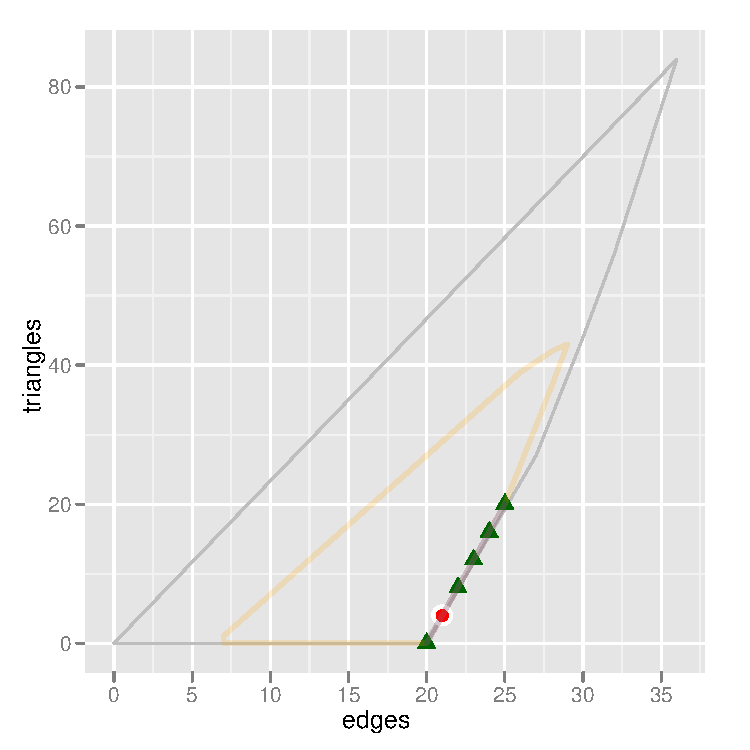
\includegraphics[height=2.5in]{MCsample-fakeface}
%\caption{MCMC samples when MLE does not exist.}
%\label{F:MCsample-MLE problem}
%\end{figure}
%}

\end{document}
